% Options for packages loaded elsewhere
\PassOptionsToPackage{unicode}{hyperref}
\PassOptionsToPackage{hyphens}{url}
\PassOptionsToPackage{dvipsnames,svgnames,x11names}{xcolor}
%
\documentclass[
  letterpaper,
]{book}

\usepackage{amsmath,amssymb}
\usepackage{iftex}
\ifPDFTeX
  \usepackage[T1]{fontenc}
  \usepackage[utf8]{inputenc}
  \usepackage{textcomp} % provide euro and other symbols
\else % if luatex or xetex
  \usepackage{unicode-math}
  \defaultfontfeatures{Scale=MatchLowercase}
  \defaultfontfeatures[\rmfamily]{Ligatures=TeX,Scale=1}
\fi
\usepackage{lmodern}
\ifPDFTeX\else  
    % xetex/luatex font selection
\fi
% Use upquote if available, for straight quotes in verbatim environments
\IfFileExists{upquote.sty}{\usepackage{upquote}}{}
\IfFileExists{microtype.sty}{% use microtype if available
  \usepackage[]{microtype}
  \UseMicrotypeSet[protrusion]{basicmath} % disable protrusion for tt fonts
}{}
\makeatletter
\@ifundefined{KOMAClassName}{% if non-KOMA class
  \IfFileExists{parskip.sty}{%
    \usepackage{parskip}
  }{% else
    \setlength{\parindent}{0pt}
    \setlength{\parskip}{6pt plus 2pt minus 1pt}}
}{% if KOMA class
  \KOMAoptions{parskip=half}}
\makeatother
\usepackage{xcolor}
\setlength{\emergencystretch}{3em} % prevent overfull lines
\setcounter{secnumdepth}{5}
% Make \paragraph and \subparagraph free-standing
\ifx\paragraph\undefined\else
  \let\oldparagraph\paragraph
  \renewcommand{\paragraph}[1]{\oldparagraph{#1}\mbox{}}
\fi
\ifx\subparagraph\undefined\else
  \let\oldsubparagraph\subparagraph
  \renewcommand{\subparagraph}[1]{\oldsubparagraph{#1}\mbox{}}
\fi


\providecommand{\tightlist}{%
  \setlength{\itemsep}{0pt}\setlength{\parskip}{0pt}}\usepackage{longtable,booktabs,array}
\usepackage{calc} % for calculating minipage widths
% Correct order of tables after \paragraph or \subparagraph
\usepackage{etoolbox}
\makeatletter
\patchcmd\longtable{\par}{\if@noskipsec\mbox{}\fi\par}{}{}
\makeatother
% Allow footnotes in longtable head/foot
\IfFileExists{footnotehyper.sty}{\usepackage{footnotehyper}}{\usepackage{footnote}}
\makesavenoteenv{longtable}
\usepackage{graphicx}
\makeatletter
\def\maxwidth{\ifdim\Gin@nat@width>\linewidth\linewidth\else\Gin@nat@width\fi}
\def\maxheight{\ifdim\Gin@nat@height>\textheight\textheight\else\Gin@nat@height\fi}
\makeatother
% Scale images if necessary, so that they will not overflow the page
% margins by default, and it is still possible to overwrite the defaults
% using explicit options in \includegraphics[width, height, ...]{}
\setkeys{Gin}{width=\maxwidth,height=\maxheight,keepaspectratio}
% Set default figure placement to htbp
\makeatletter
\def\fps@figure{htbp}
\makeatother
% definitions for citeproc citations
\NewDocumentCommand\citeproctext{}{}
\NewDocumentCommand\citeproc{mm}{%
  \begingroup\def\citeproctext{#2}\cite{#1}\endgroup}
\makeatletter
 % allow citations to break across lines
 \let\@cite@ofmt\@firstofone
 % avoid brackets around text for \cite:
 \def\@biblabel#1{}
 \def\@cite#1#2{{#1\if@tempswa , #2\fi}}
\makeatother
\newlength{\cslhangindent}
\setlength{\cslhangindent}{1.5em}
\newlength{\csllabelwidth}
\setlength{\csllabelwidth}{3em}
\newenvironment{CSLReferences}[2] % #1 hanging-indent, #2 entry-spacing
 {\begin{list}{}{%
  \setlength{\itemindent}{0pt}
  \setlength{\leftmargin}{0pt}
  \setlength{\parsep}{0pt}
  % turn on hanging indent if param 1 is 1
  \ifodd #1
   \setlength{\leftmargin}{\cslhangindent}
   \setlength{\itemindent}{-1\cslhangindent}
  \fi
  % set entry spacing
  \setlength{\itemsep}{#2\baselineskip}}}
 {\end{list}}
\usepackage{calc}
\newcommand{\CSLBlock}[1]{\hfill\break\parbox[t]{\linewidth}{\strut\ignorespaces#1\strut}}
\newcommand{\CSLLeftMargin}[1]{\parbox[t]{\csllabelwidth}{\strut#1\strut}}
\newcommand{\CSLRightInline}[1]{\parbox[t]{\linewidth - \csllabelwidth}{\strut#1\strut}}
\newcommand{\CSLIndent}[1]{\hspace{\cslhangindent}#1}

\usepackage{fancyhdr}
\usepackage{graphicx}
\usepackage{eso-pic}
\usepackage{tikz}
\AtBeginDocument{\thispagestyle{empty}\begin{tikzpicture}[remember picture,overlay] \node at (current page.center) [yshift=1cm] {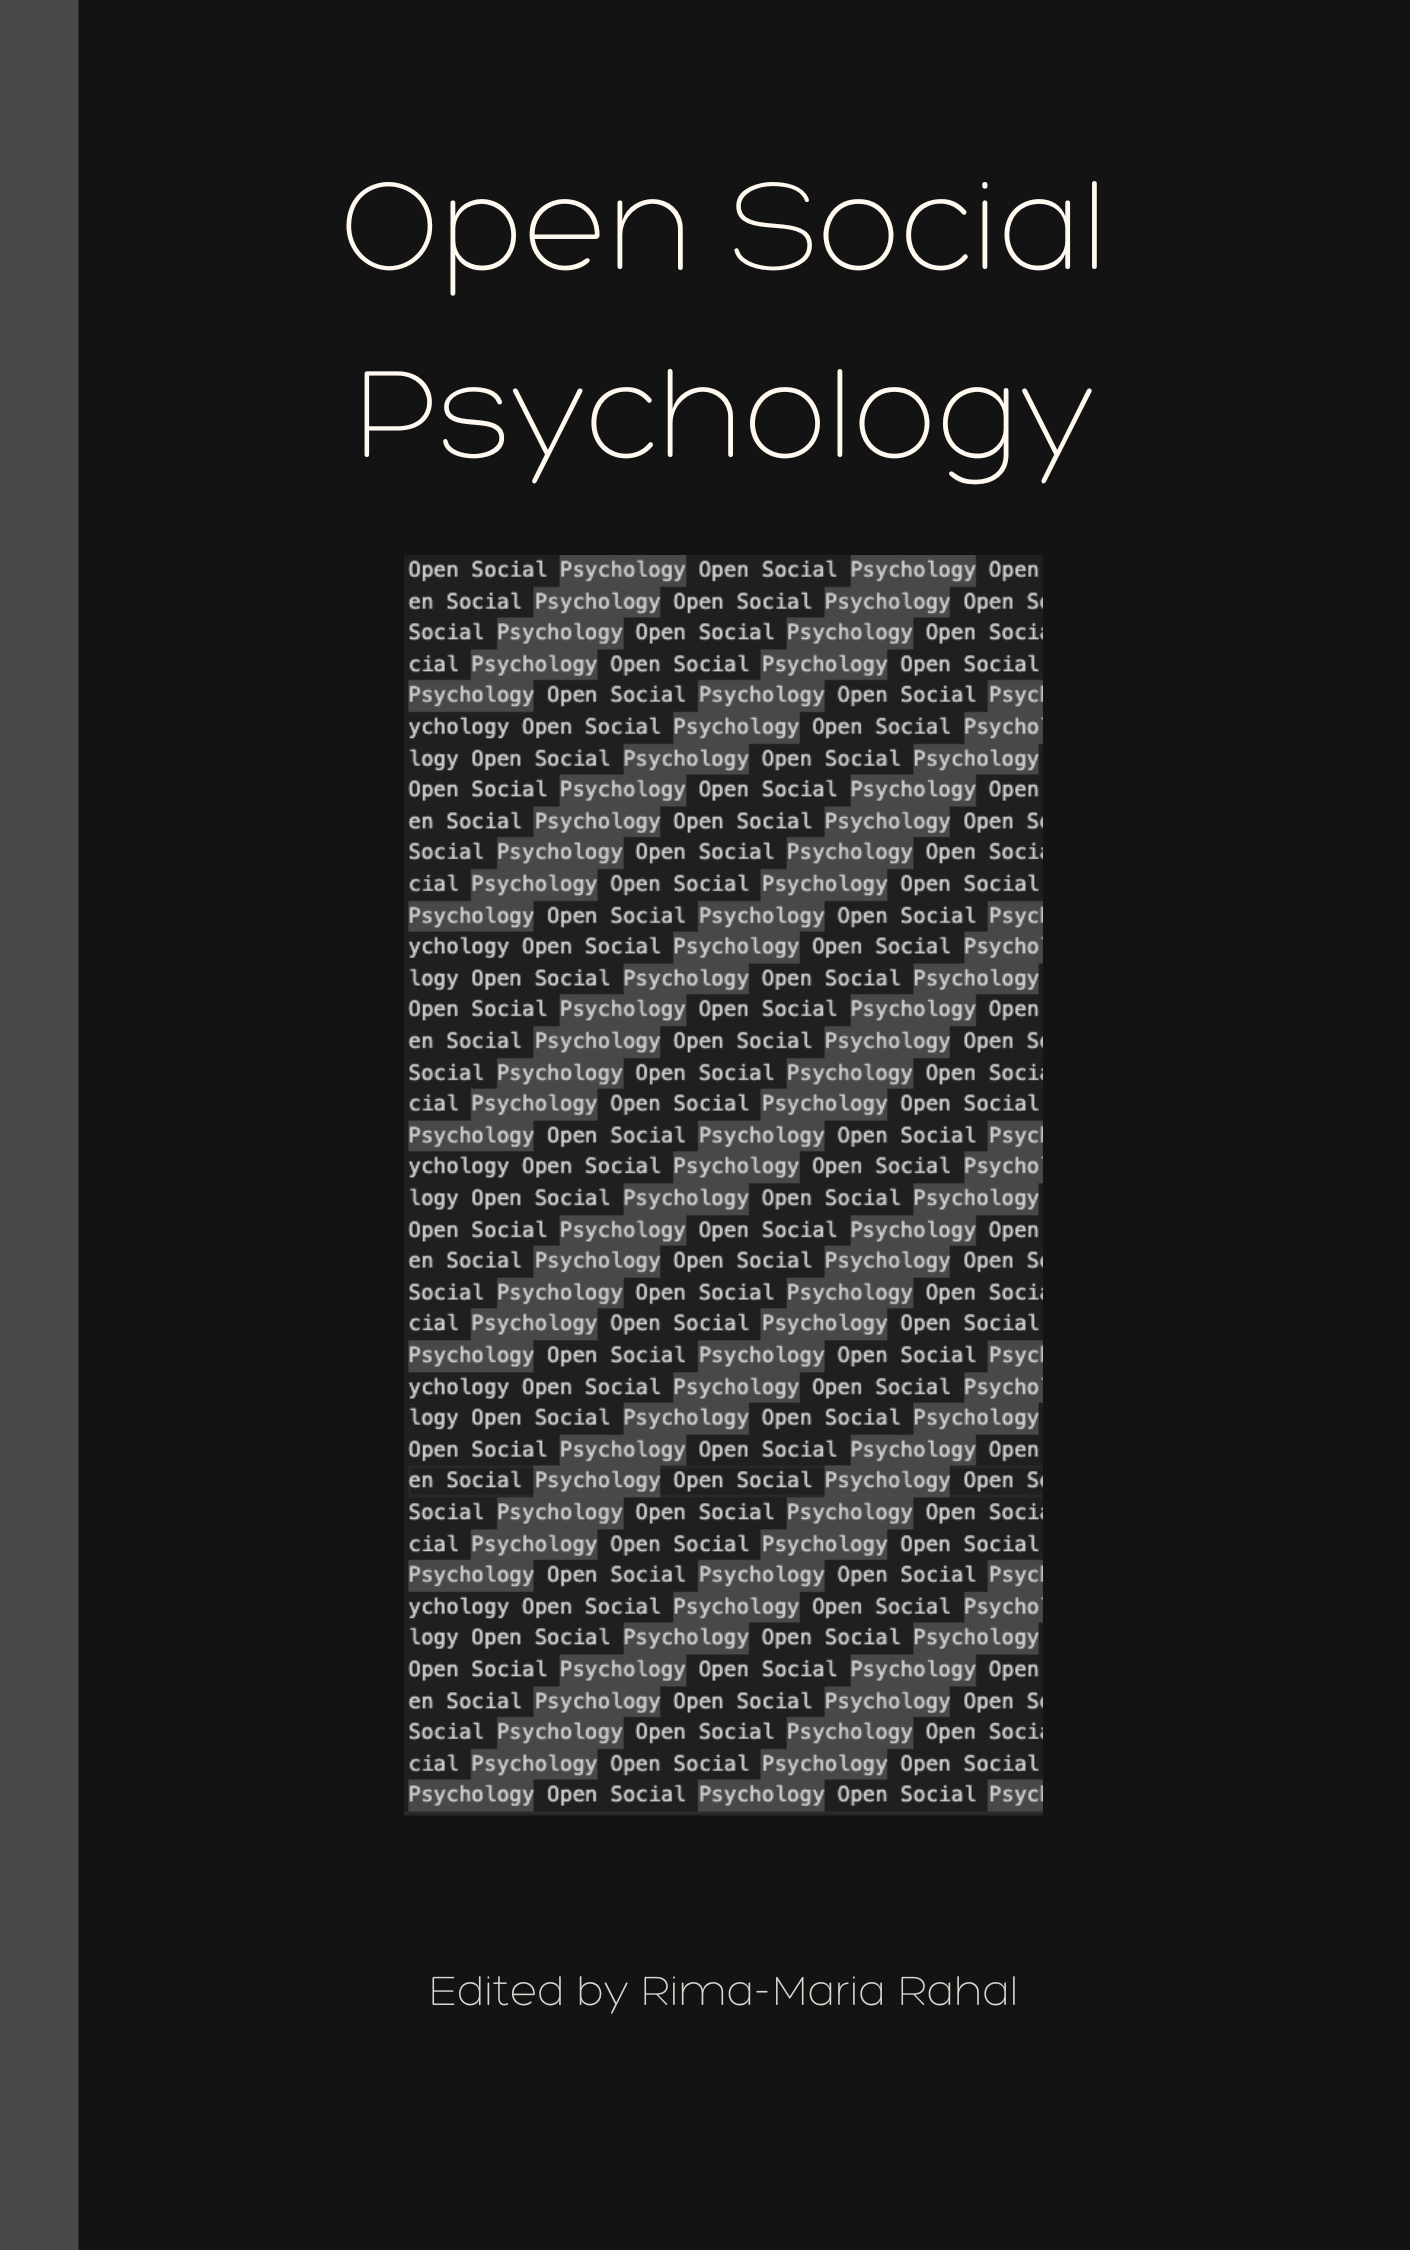
\includegraphics[width=0.75\paperwidth,height=0.9\paperheight,keepaspectratio]{resources/cover.png}}; \end{tikzpicture}\clearpage}
\makeatletter
\@ifpackageloaded{bookmark}{}{\usepackage{bookmark}}
\makeatother
\makeatletter
\@ifpackageloaded{caption}{}{\usepackage{caption}}
\AtBeginDocument{%
\ifdefined\contentsname
  \renewcommand*\contentsname{Table of contents}
\else
  \newcommand\contentsname{Table of contents}
\fi
\ifdefined\listfigurename
  \renewcommand*\listfigurename{List of Figures}
\else
  \newcommand\listfigurename{List of Figures}
\fi
\ifdefined\listtablename
  \renewcommand*\listtablename{List of Tables}
\else
  \newcommand\listtablename{List of Tables}
\fi
\ifdefined\figurename
  \renewcommand*\figurename{Figure}
\else
  \newcommand\figurename{Figure}
\fi
\ifdefined\tablename
  \renewcommand*\tablename{Table}
\else
  \newcommand\tablename{Table}
\fi
}
\@ifpackageloaded{float}{}{\usepackage{float}}
\floatstyle{ruled}
\@ifundefined{c@chapter}{\newfloat{codelisting}{h}{lop}}{\newfloat{codelisting}{h}{lop}[chapter]}
\floatname{codelisting}{Listing}
\newcommand*\listoflistings{\listof{codelisting}{List of Listings}}
\makeatother
\makeatletter
\makeatother
\makeatletter
\@ifpackageloaded{caption}{}{\usepackage{caption}}
\@ifpackageloaded{subcaption}{}{\usepackage{subcaption}}
\makeatother
\ifLuaTeX
  \usepackage{selnolig}  % disable illegal ligatures
\fi
\usepackage{bookmark}

\IfFileExists{xurl.sty}{\usepackage{xurl}}{} % add URL line breaks if available
\urlstyle{same} % disable monospaced font for URLs
\hypersetup{
  pdftitle={Open Social Psychology},
  pdfauthor={Rima-Maria Rahal},
  colorlinks=true,
  linkcolor={green},
  filecolor={Maroon},
  citecolor={green},
  urlcolor={Blue},
  pdfcreator={LaTeX via pandoc}}

\title{Open Social Psychology}
\author{Rima-Maria Rahal}
\date{2025-02-05}

\begin{document}
\frontmatter
\maketitle

\renewcommand*\contentsname{Table of contents}
{
\hypersetup{linkcolor=}
\setcounter{tocdepth}{2}
\tableofcontents
}
\mainmatter
\bookmarksetup{startatroot}

\chapter*{\texorpdfstring{{Preface}}{Preface}}\label{preface}
\addcontentsline{toc}{chapter}{{Preface}}

\markboth{{Preface}}{{Preface}}

Social psychology is built on a strong set of classical research
paradigms and findings, featured in many of the textbooks, syllabi,
online courses and teaching guides that aspiring psychologists study
with and established psychologists use as teaching resources. However,
the common body of knowledge that social psychology relies on is
undergoing change. Modern research methods and changing attitudes
towards permissible research practices bring about social psychological
research that looks different today than it used. This book is dedicated
to tracing some of these changes, and to offering a version of record of
the changing perceptions and interpretations of classic social
psychology in the light of it's contemporary counterpart. As such, this
study book is a snapshot of how we see social psychology today.

Because it tends to be difficult to keep teaching and study materials up
to date with emerging trends and debates, we see this study book as an
addition to traditional educational resources in social psychology. It
is published as an Open Educational Resource to aid the accessibility of
this knowledge for all, and to be adapted to teachers' and learners'
needs as they dive into what social psychology has to offer.

\bookmarksetup{startatroot}

\chapter*{\texorpdfstring{{How this Book Came to
Be}}{How this Book Came to Be}}\label{how-this-book-came-to-be}
\addcontentsline{toc}{chapter}{{How this Book Came to Be}}

\markboth{{How this Book Came to Be}}{{How this Book Came to Be}}

{written by Flávio Azevedo and Rima-Maria Rahal}

Social psychology is devoted to studying how individuals behave, think
and feel within their social contexts. The field is therefore, by its
very nature, set up for collaborative work. Leveraging the social
context in which knowledge is generated is built in to the assumptions
and interests that social psychology pursues. This fundamental attitude
towards social embeddedness of knowledge is mirrored in the process by
which this study book came to be.

It started by bringing together the work of students at Heidelberg
University during the winter term of 2023. In the scope of classwork,
they engaged with classical findings of social psychology, and discussed
recent attempts to reengage with these classics. These works are the
basis of the current book.

Researchers working on (areas related to) social psychology then revised
these chapters. Through engaging the communities at the Big Team Science
Conference 2024
(\href{https://bigteamscienceconference.github.io}{BTScon}), and the
Framework for Open and Reproducible Research Training
(\href{https://forrt.org}{FORRT}), we found collaborators willing to
contribute their knowledge and expertise to turning chapter drafts into
an approachable and fact checked resource.

Consequently, this volume offers diverse perspectives on a shared target
topic: Changing perceptions of classical social psychological research.

\bookmarksetup{startatroot}

\chapter*{\texorpdfstring{{How to Use this
Book}}{How to Use this Book}}\label{how-to-use-this-book}
\addcontentsline{toc}{chapter}{{How to Use this Book}}

\markboth{{How to Use this Book}}{{How to Use this Book}}

{written by Melissa Engelbart and Rima-Maria Rahal}

This book contains several types of resources: narrative text,
definitions and questions for reflection, as well as references.

In fifteen chapters, we provide narrative summaries about classical
research in social psychology and its modern follow-up. Often, this
means we include new attempts to show the same finding (replication
attempts) or meta-analytical work that brings together a lot of evidence
from different sources regarding a certain hypothesis. Each chapter
contains an overview of the classic study, a summary of important work
thereafter, as well as a discussion of the evidence, experiments or
analyses conducted. We then attempt to draw conclusions about the tested
hypotheses.

Because this volume is targeted at students, we provide definitions of
key terms, preceded by {\#definition} and displayed like this:

\begin{quote}
{\#definition} Replication

An attempt to find the same result as a previous study in a new data
set.
\end{quote}

\begin{quote}
{\#definition} Meta-Analysis

An analysis that brings together evidence from several individual
studies or experiments to estimate an overall effect across the
available evidence.
\end{quote}

We have aimed at providing a critical but neutral perspective to the
classical and modern studies of social psychology discussed in the texts
of this volume. To help you develop your own perspective and a
well-reflected attitude towards this work, you will find guiding
questions and suggestions that might prompt you to think more deeply
about what you read throughout the book. The guiding questions cover
topics such as the research and publication process itself and it's
influence on research, the interpretation of data in general, as well as
the experimental operationalization of theoretical questions. Moreover,
to help you consider potential applications of the findings and theories
discussed, these questions sometimes ask you to think of examples or
consequences in real life.

You'll recognize these prompts by the preceding {\#yourturn.} Here is an
example of what these questions look like:

\begin{quote}
{\#yourturn}

Do you think you might find such questions for reflection useful?
\end{quote}

Finally, we have enabled the option to collaboratively annotate this
work using \href{https://web.hypothes.is/}{hypothesis} (note that this
is how links are formatted in this book) in the online version. Your
annotations will be visible to others, and others will be able to see
yours, so that we can build a better learning experience using this book
together.

To read up on the original research we cite in this book, such as from
Vazire (\citeproc{ref-vazire2018}{2018}), you can hover over or click on
the references provided.

Feel free to make use of the resources in this book as you see fit. Our
hope is that they will support you in building a well-reflected opinion
about the existing body of knowledge in social psychology.

\bookmarksetup{startatroot}

\chapter*{\texorpdfstring{{Introduction}}{Introduction}}\label{introduction}
\addcontentsline{toc}{chapter}{{Introduction}}

\markboth{{Introduction}}{{Introduction}}

\section*{The Role of Change for Scientific
Discovery}\label{the-role-of-change-for-scientific-discovery}
\addcontentsline{toc}{section}{The Role of Change for Scientific
Discovery}

\markright{The Role of Change for Scientific Discovery}

Much of science capitalizes on change. It is the engine that drives
progress and the expansion of knowledge (see
\citeproc{ref-kuhn1962structure}{Kuhn 1962};
\citeproc{ref-popper1959logic}{Popper 1959}). Embracing change means
taking established theories and challenging them to explore new
directions. Changing perspectives, questioning the status quo, refining
existing concepts, and adapting to new evidence provide the stuff that
makes breakthroughs or new insights. In essence, change in science
represents taking steps forward, toward greater insight and reality
checks for the challenges we face. In other words, to push the
boundaries of what we know, we must make change.

\begin{quote}
{\#yourturn}

What instance of change regarding science have you recently heard about?
Consider reports of breakthroughs you might have seen in the news or
stories you saw on social media.
\end{quote}

In the past decade, Open Science has made change, by transforming
research practices to promote transparency, reproducibility, and
collaboration in scientific endeavors. By fostering a culture of
openness and collaboration, Open Science has brought about a paradigm
shift in research methodologies, paving the way for more robust and
reliable scientific discoveries
(\citeproc{ref-munafo2017manifesto}{Munafò et al. 2017};
\citeproc{ref-vazire2022credibility}{Vazire, Schiavone, and Bottesini
2022}). It is certainly no small feat to fundamentally reform how
research is done, and yet we have seen significant change towards Open
practices (\citeproc{ref-kidwell2016badges}{Kidwell et al. 2016};
\citeproc{ref-chambers2019registered}{Chambers 2019};
\citeproc{ref-christensen2020open}{Christensen et al. 2020}).

\begin{quote}
{\#definition} Open Science

An overhead term for a number of practices to make research more
transparent, such as making the data a research is project is based on
available to others.
\end{quote}

\section*{Challenges of Making
Change}\label{challenges-of-making-change}
\addcontentsline{toc}{section}{Challenges of Making Change}

\markright{Challenges of Making Change}

Change can be a challenge because it disrupts established norms, habits,
and power structures. This often means that individuals and groups might
be hesitant to embrace change. Open Science as a reform to refocus on
good research practice had to work with this difficulty of making
change, where new methods, theories, or technologies often encounter
skepticism and opposition from the scientific community. Open Science
promotes transparency, data sharing, and collaborative research, which
can expose flaws underlying previously held beliefs or reveal
alternative interpretations. This shift can create debates about
long-held ideas and established practices, which are scrutinized and
potentially overturned. Established researchers may be reluctant to
abandon familiar paradigms, and institutions may resist reallocating
resources or altering well-known processes. Sometimes, inertia of
traditional practices and fear of uncertainty can slow the adoption of
innovative approaches, despite their potential to advance knowledge and
solve pressing problems.

\begin{quote}
{\#yourturn}

Consider a big change you have experienced. Was it easy to adapt to this
change?
\end{quote}

However, a questioning attitude and focus on methodological rigor and
good practice also enhance the robustness and reliability of scientific
conclusions by fostering an environment where continuous re-evaluation
is encouraged. Thus, Open Science exemplifies how embracing change can
lead to a more dynamic and resilient understanding of the world, even as
it unsettles the familiar foundations of scientific consensus.

Change often implies the potential for a changed perception of what used
to be, particularly in comparison to what is now. This is also the case
in the scope of changes assosciated with Open Science. In particular,
what were once considered unassailable facts can become contested or
uncertain as new methodologies, data, and technologies challenge
established knowledge. This is where our focus lies in this book:
reporting on classical studies in social psychology and the change in
how they are seen now, following a wave of additional research (often
with an Open Science flavor).

\begin{quote}
{\#yourturn}

``I was today years old when I found out \ldots{}'' What was the last
long-held belief you had to give up?
\end{quote}

In this spirit, when reading about the changes in perspective about
classics in social psychology, there are two things to embrace:

On the one hand, revisiting classic social psychology studies is a
demonstration on the profound impact they had on the field. Were they
less important and less impactful, these studies would not draw
continued debate, research interest and investment of resources.
Therefore, reading classic studies can give readers a sense of what
matters to social psychological research, from hot topics to hot
paradigms and research methods.

On the other hand, following the course of the academic debate about
these claims, insights and phenomena allows us to hone our skills in
accumulating insights and adjusting our perception of the currently held
beliefs in this area of research. Put differently, tracing efforts to
replicate, to conduct meta-analyses or to establish boundary conditions
to the findings postulated in a certain study mostly reflects
well-intentioned interest in assessing the validity of the claims of the
original study, attempting to produce clarity about our collective
knowledge about the phenomenon of interest. Reassessing classical
studies might require change in opinions, calibration and reflection,
but it can surely spark renewed trust in research and in its ability to
refine and build our joint knowledge.

\bookmarksetup{startatroot}

\chapter{\texorpdfstring{{Ego
Depletion}}{Ego Depletion}}\label{ego-depletion}

{written by Hannah Baumgart and Rima-Maria Rahal}

\section{The Classic}\label{the-classic}

Ego depletion is a social psychological concept that describes the
depletion of individuals' self-regulatory resources. Baumeister et al.
(\citeproc{ref-baumeister1998}{1998}) were the first to demonstrate ego
depletion effects in four different experimental settings: After having
to engage in an act of self-control (compared to a control task that
does not require self-control), willpower is used up and could not be
deployed as effectively in a subsequent task.

\begin{quote}
\phantomsection\label{def-egodepletion}{\#definition} Ego Depletion

A concept that describes willpower as a limited resource that can be
used up (depleted).
\end{quote}

In Experiment 1, the focus was on the act of resisting a temptation,
which requires self-control. Participants were randomly assigned to
different food conditions, by which the independent variables were
manipulated: Chocolate chip cookies and chocolate, radishes or no food
at all (control group). Participants in the radish control condition
were instructed to resist the tempting chocolates and instead eat
several the radishes that were laid out next to the chocolate. In the
chocolate condition, participants were asked to eat several cookies or
chocolates, which were laid out next to the radishes -- a task that was
not supposed to require much self-control. The actual intention behind
the experiment, to demonstrate ego depletion, was disguised with a cover
story to make sure participants would not get suspicious. They were told
the experiment was about taste perception.

\begin{quote}
{\#yourturn}

Which other tasks in your daily life require more or less willpower?
\end{quote}

In the no-food control condition, participants were not asked to taste
any food, but worked on the rest of the experiment.

After the participants had completed the willpower task resisting the
temptation of the foods presented to them, they had to complete
questionnaires on mood and restraint. Then they had to work on
``solving'' a problem-solving task, which was actually unsolvable. Here,
the time spent on trying to solve the problem before giving up was the
dependent variable.

The results showed significant differences between the three conditions,
with participants in the radish condition stopping earlier than those in
the chocolate or no-food condition. In conclusion, it was suggested that
craving chocolate but choosing to eat radishes depleted an internal
resource, leaving individuals less able to persist while trying to solve
the puzzles afterwards.

\begin{quote}
{\#yourturn}

If willpower can be depleted, how can it be ``refilled'' or built up
again?
\end{quote}

\section{The Aftermath}\label{the-aftermath}

Since this study, several hundred follow-up studies, including several
multi-lab studies that aimed to replicate the overall finding
(\citeproc{ref-hagger2010}{Hagger et al. 2010};
\citeproc{ref-vohs2021}{Vohs et al. 2021}) and several meta-analyses
(\citeproc{ref-hagger2010}{Hagger et al. 2010};
\citeproc{ref-carter2014}{Carter and McCullough 2014};
\citeproc{ref-dang2017a}{Dang 2017};
\citeproc{ref-bluxe1zquez2017}{Blázquez, Botella, and Suero 2017}) have
been carried out.

\begin{quote}
\phantomsection\label{def-multilabstudy}{\#definition} Multi-Lab Study

A research project in which researchers working at several different
locations (laboratories) implement the same experimental design and then
analyse the data together.
\end{quote}

These studies yielded mixed results, with some concluding that it was
highly unlikely that the ego depletion phenomenon does not exist (e.g.,
\citeproc{ref-hagger2010}{Hagger et al. 2010}), while others failed to
establish the effect despite relying on data from more than 2000
participants (e.g., \citeproc{ref-hagger2010}{Hagger et al. 2010}).
Publication bias has been argued to be high in the literature on ego
depletion (\citeproc{ref-inzlicht2015}{Inzlicht, Gervais, and Berkman
2015}), casting doubt on the effect.

\begin{quote}
{\#definition} Publication Bias

A tendency for research in line with established theories or showing
significant results to be more easily publishable than deviating
research.
\end{quote}

Continued research interest on ego depletion has brought forward varying
hypotheses regarding circumstances under which the effect might be
demonstrable and robust. The meta-analysis on ego depletion conducted by
Dang (\citeproc{ref-dang2017a}{2017}) investigated only studies with
sufficient initial effort exerted in the depleting, which was
hypothesized to lead to the ego depletion effect. The study ensured that
the depleting task required the use of self-control and excluded
manipulations that were less clearly related to self-control, such as
those based on social exclusion. Eight commonly used depletion tasks
were assessed in the meta-analysis: attention essay, attention video,
crossing out letters, emotion video, food trial, Stroop, thought
suppression, and working memory.

\begin{quote}
{\#yourturn}

Can you imagine what participants had to do in these tasks? Think about
a version of each task that would drain self-control and one that would
be less exhausting.
\end{quote}

The results showed that two of these exhausting tasks, attention video
and working memory, were not associated with significant changes in
subsequent self-control. Emotion videos, on the other hand, appeared to
be the most effective task and reduced subsequent self-control.

The overall analysis revealed a small to medium effect size for the ego
depletion effect. Correcting for publication bias, this effect was not
statistically significant when using the full sample of studies
identified. However, a separate analysis for reliable depletion tasks,
such as attention essay, emotion video and Stroop, showed the
significant effect remained when attempting to correct for publication
bias. This meta-analysis suggests that in special tasks, ego depletion
might occur, but that it is difficult to generalize to other
circumstances.

However, even in these special tasks, there is often no direct measure
of the initial depletion of willpower involved: manipulation checks on
whether willpower has been used up offer only an indirect measurement
(\citeproc{ref-friese2018}{Friese et al. 2018}).

\begin{quote}
{\#yourturn}

How could you objectiveley measure the amount of willpower available or
drained?
\end{quote}

\section{Conclusion}\label{conclusion}

The literature suggests a differentiated view on the potentially finite
nature of willpower is necessary (for a detailed overview, read more in
\citeproc{ref-friese2018}{Friese et al. 2018}). In the context of social
psychological theories, the ego depletion effect can be seen as an
important example of contradictory findings in research, where
publication bias may play a role. Although several hundred studies on
ego depletion have been published, we cannot be sure whether ego
depletion exists or not.

\begin{quote}
{\#yourturn}

Do you think ego depletion exists?
\end{quote}

The debate about ego depletion shows that individual findings should be
reassessed in several empirical demonstrations, including replication
attempts that can provide a more realistic picture of the effect or
construct. In this case, the original ego depletion effect may have been
initially inflated due to publication bias. Following closer
examination, it is less certain whether this effect indeed exists. The
example of the ego depletion literature also shows the importance of
examining the evidence closely, under the microscope, in order to ensure
that it meets the quality criteria that are essential for assessing
cumulative evidence of the overall effect.

\bookmarksetup{startatroot}

\chapter*{\texorpdfstring{{Summary}}{Summary}}\label{summary}
\addcontentsline{toc}{chapter}{{Summary}}

\markboth{{Summary}}{{Summary}}

Add here

\section*{Take-Aways}\label{take-aways}
\addcontentsline{toc}{section}{Take-Aways}

\markright{Take-Aways}

Add here

\section*{Thanks}\label{thanks}
\addcontentsline{toc}{section}{Thanks}

\markright{Thanks}

This book was made possible by the many helping hands and critical
thoughts of the student authors involved in writing the individual
chapters. In addition, Melissa Engelbarth's support with selecting and
translating the chapters to include was invaluable.

\bookmarksetup{startatroot}

\chapter*{References}\label{references}
\addcontentsline{toc}{chapter}{References}

\markboth{References}{References}

\phantomsection\label{refs}
\begin{CSLReferences}{1}{0}
\bibitem[\citeproctext]{ref-baumeister1998}
Baumeister, Roy F., Ellen Bratslavsky, Mark Muraven, and Dianne M. Tice.
1998. {``Ego Depletion: Is the Active Self a Limited Resource?''}
\emph{Journal of Personality and Social Psychology} 74 (5): 1252--65.
\url{https://doi.org/10.1037/0022-3514.74.5.1252}.

\bibitem[\citeproctext]{ref-bluxe1zquez2017}
Blázquez, Desirée, Juan Botella, and Manuel Suero. 2017. {``The Debate
on the Ego-Depletion Effect: Evidence from Meta-Analysis with the
p-Uniform Method.''} \emph{Frontiers in Psychology} 8 (February).
\url{https://doi.org/10.3389/fpsyg.2017.00197}.

\bibitem[\citeproctext]{ref-carter2014}
Carter, Evan C., and Michael E. McCullough. 2014. {``Publication Bias
and the Limited Strength Model of Self-Control: Has the Evidence for Ego
Depletion Been Overestimated?''} \emph{Frontiers in Psychology} 5
(July). \url{https://doi.org/10.3389/fpsyg.2014.00823}.

\bibitem[\citeproctext]{ref-chambers2019registered}
Chambers, Chris. 2019. {``The Registered Reports Revolution Lessons in
Cultural Reform.''} \emph{Significance} 16 (4): 23--27.

\bibitem[\citeproctext]{ref-christensen2020open}
Christensen, Garret, Zenan Wang, Elizabeth Levy Paluck, Nicholas
Swanson, David Birke, Edward Miguel, and Rebecca Littman. 2020. {``Open
Science Practices Are on the Rise: The State of Social Science (3S)
Survey.''}

\bibitem[\citeproctext]{ref-dang2017a}
Dang, Junhua. 2017. {``An Updated Meta-Analysis of the Ego Depletion
Effect.''} \emph{Psychological Research} 82 (4): 645--51.
\url{https://doi.org/10.1007/s00426-017-0862-x}.

\bibitem[\citeproctext]{ref-friese2018}
Friese, Malte, David D. Loschelder, Karolin Gieseler, Julius
Frankenbach, and Michael Inzlicht. 2018. {``Is Ego Depletion Real? An
Analysis of Arguments.''} \emph{Personality and Social Psychology
Review} 23 (2): 107--31. \url{https://doi.org/10.1177/1088868318762183}.

\bibitem[\citeproctext]{ref-hagger2010}
Hagger, Martin S., Chantelle Wood, Chris Stiff, and Nikos L. D.
Chatzisarantis. 2010. {``Ego Depletion and the Strength Model of
Self-Control: A Meta-Analysis.''} \emph{Psychological Bulletin} 136 (4):
495--525. \url{https://doi.org/10.1037/a0019486}.

\bibitem[\citeproctext]{ref-inzlicht2015}
Inzlicht, Michael, Will Gervais, and Elliot Berkman. 2015.
{``Bias-Correction Techniques Alone Cannot Determine Whether Ego
Depletion Is Different from Zero: Commentary on Carter, Kofler, Forster,
\& Mccullough, 2015.''} \emph{SSRN Electronic Journal}.
\url{https://doi.org/10.2139/ssrn.2659409}.

\bibitem[\citeproctext]{ref-kidwell2016badges}
Kidwell, Mallory C, Ljiljana B Lazarević, Erica Baranski, Tom E
Hardwicke, Sarah Piechowski, Lina-Sophia Falkenberg, Curtis Kennett, et
al. 2016. {``Badges to Acknowledge Open Practices: A Simple, Low-Cost,
Effective Method for Increasing Transparency.''} \emph{PLoS Biology} 14
(5): e1002456.

\bibitem[\citeproctext]{ref-kuhn1962structure}
Kuhn, Thomas. 1962. {``The Structure of Scientific Revolutions.''}
\emph{International Encyclopedia of Unified Science} 2 (2).

\bibitem[\citeproctext]{ref-munafo2017manifesto}
Munafò, Marcus R, Brian A Nosek, Dorothy VM Bishop, Katherine S Button,
Christopher D Chambers, Nathalie Percie du Sert, Uri Simonsohn, Eric-Jan
Wagenmakers, Jennifer J Ware, and John Ioannidis. 2017. {``A Manifesto
for Reproducible Science.''} \emph{Nature Human Behaviour} 1 (1): 1--9.

\bibitem[\citeproctext]{ref-popper1959logic}
Popper, Karl R. 1959. \emph{The Logic of Scientific Discovery}.
Hutchinson \& Co.

\bibitem[\citeproctext]{ref-vazire2018}
Vazire, Simine. 2018. {``Implications of the Credibility Revolution for
Productivity, Creativity, and Progress.''} \emph{Perspectives on
Psychological Science} 13 (4): 411--17.
\url{https://doi.org/10.1177/1745691617751884}.

\bibitem[\citeproctext]{ref-vazire2022credibility}
Vazire, Simine, Sarah R Schiavone, and Julia G Bottesini. 2022.
{``Credibility Beyond Replicability: Improving the Four Validities in
Psychological Science.''} \emph{Current Directions in Psychological
Science} 31 (2): 162--68.

\bibitem[\citeproctext]{ref-vohs2021}
Vohs, Kathleen D., Brandon J. Schmeichel, Sophie Lohmann, Quentin F.
Gronau, Anna J. Finley, Sarah E. Ainsworth, Jessica L. Alquist, et al.
2021. {``A Multisite Preregistered Paradigmatic Test of the
Ego-Depletion Effect.''} \emph{Psychological Science} 32 (10): 1566--81.
\url{https://doi.org/10.1177/0956797621989733}.

\end{CSLReferences}

\bookmarksetup{startatroot}

\chapter*{\texorpdfstring{{Glossary}}{Glossary}}\label{glossary}
\addcontentsline{toc}{chapter}{{Glossary}}

\markboth{{Glossary}}{{Glossary}}

In this glossary, you can find the terms defined in this book in
alphabetical order.

\subsubsection*{\texorpdfstring{\hyperref[def-egodepletion]{Ego
Depletion}}{Ego Depletion}}\label{ego-depletion-1}
\addcontentsline{toc}{subsubsection}{\hyperref[def-egodepletion]{Ego
Depletion}}

A concept that describes willpower as a limited resource that can be
used up (depleted).

\subsubsection*{\texorpdfstring{\hyperref[def-multilabstudy]{Multi-Lab
Study}}{Multi-Lab Study}}\label{multi-lab-study}
\addcontentsline{toc}{subsubsection}{\hyperref[def-multilabstudy]{Multi-Lab
Study}}

A research project in which researchers working at several different
locations (laboratories) implement the same experimental design and then
analyse the data together.


\backmatter

\end{document}
